\documentclass{article}
\usepackage[T1]{fontenc}
% The local Tectonic cache lacks cmbx12.tfm; map it to the cached LM glyphs.
\DeclareFontShape{OT1}{cmr}{bx}{n}{<-> ec-lmbx12}{}
\usepackage{iclr2026_conference,times}
\usepackage{amsmath,amssymb,booktabs,graphicx,tabularx,url}
\usepackage{hyperref}
\hypersetup{hidelinks}
\raggedbottom
% Table captions sit above the \toprule; article's default \belowcaptionskip=0pt let the
% caption's descenders touched the rule in a prior page render.
\setlength{\belowcaptionskip}{5pt}

% r240 layout audit: the title is a justified paragraph in the style file, and its first
% line could only break before the 8-character word "Accuracy", which stretched the three
% word spaces of line 1 to roughly three times their natural width (underfull \hbox
% badness 10000 at this line).  The wording is unchanged; the breaks below are the ones
% TeX already chose, now taken explicitly so each line is set at natural word spacing.
\title{Length-Associated Signed Confidence--\\Accuracy Gaps: An Observational Decomposition,\\a Within-Item Causal Check, and\\a Human-Anchored Cross-Bed Sensitivity}
\author{Anonymous authors}
\date{}

\begin{document}
\maketitle
\lhead[Under review as a conference paper at ICLR 2026]{Under review as a conference paper at ICLR 2026}

\begin{abstract}
We study how prompt length relates to the signed confidence--accuracy gap in
masked-diffusion decoding and whether that relationship is causal.  On GSM8K with
LLaDA-8B-Instruct, the observational contrast across prompt-length variants is
$+0.2227$ with a primary 95\% cluster-bootstrap interval $[0.169,0.277]$.
An exact two-component decomposition shows that accuracy falls much faster than
confidence.  In a randomized within-item experiment with $400$ paired problems,
content-free redundant filler, and a fixed decode budget, the signed-gap contrast is
$-0.0075$ [$\,{-}0.052,+0.039$].  At the $+37$-token intervention dose, this interval
includes zero but excludes the $+0.2227$ observational magnitude (a dose-local, not
exactly dose-matched, comparison; \S\ref{sec:calib}).  The preregistered verdict is
therefore \textsc{not\_identified}: content-free length is not detected to widen the
gap on this bed, and the observational contrast does not establish a length mechanism.
On MATH500, the post-repair v2 judge agrees with all $30$ human anchors and yields a
designated v2 estimate of $+0.2382$ [$0.1639,0.3125$].  Under the lenient judge, a
$30$-anchor pair-bias correction gives $+0.1606$ [$\,{-}0.059,+0.380$], an
anchor-dependent design sensitivity interval rather than a repeat-sampling confidence
interval.  Because that interval contains zero, cross-bed transport remains
\textsc{power\_limited} (\S\ref{sec:mdls}).  Within GSM8K, the point estimate also
decreases toward and through zero in harder outcome-defined accuracy regimes; this is a
boundary on the association, not a mechanism claim.
\end{abstract}

\section{Introduction}
\label{sec:intro}
Masked-diffusion language models decode by iteratively unmasking tokens under a
scheduled transition.  A decoder's self-reported probability when it commits an output
is a natural confidence signal for downstream use, but its relationship to correctness
may change with prompt length.  Accuracy and confidence can move in opposite directions;
their \emph{signed} gap---confidence minus correctness---therefore distinguishes a
change in confidence from a change in calibration-in-the-large.  We measure the
length-associated signed gap in a fixed GSM8K \citep{cobbe2021gsm8k} /
LLaDA-8B-Instruct \citep{nie2025large} setting and use a within-item intervention to test
whether the observed association is attributable to content-free length.  Our
contributions are:
\begin{enumerate}
\item an exact two-component decomposition $\Delta\mathrm{SCE}=\Delta\mathrm{conf}-\Delta\mathrm{acc}$
showing that the signed-gap difference is dominated by the accuracy component
(accuracy share $114.1\%$, confidence share $-14.1\%$);
\item a preregistered, within-item randomized intervention
($N{=}400$ paired problems, content-free redundant filler) that detects no causal
widening of the signed gap while bounding the effect
($[-0.052,+0.039]$) tightly enough to exclude the $+0.2227$ observational magnitude;
\item an audited answer-matching judge and a human-anchor correction on a second,
harder bed, reported conservatively as \textsc{power\_limited} with the
judge-convention dependence made explicit;
\item a traceable evidence package that links each headline number to a frozen artifact
and a one-command reproducer.
\end{enumerate}
The remainder of the paper defines the estimand and reports the single-bed
decomposition and causal check (\S\ref{sec:calib}), the second-bed read
(\S\ref{sec:calib:bed2}), the accuracy-regime boundary (\S\ref{sec:calib:control}),
the experimental setup (\S\ref{sec:setup}), the judge validation and anchor
adjudication, related work, limitations, and the reporting-layer citable read.

\section{Length-associated signed gap: the single-bed decomposition and a within-item causal check}
\label{sec:calib}

\paragraph{Definitions.}
A \emph{bed} is one fixed task--model--decoder evaluation setting.  The signed
calibration error is $\mathrm{SCE}=\mathbb{E}[\mathrm{conf}]-\mathbb{E}[\mathrm{acc}]$,
the mean commit-step confidence minus mean correctness; \emph{commit-step confidence}
is the decoder's final self-reported probability at the commit step.  The reporting
grade set is four-valued: \textsc{support} means evidence reproducible under the
predeclared audit, \textsc{power\_limited} means not established (here because of
human-anchor volume, not GPU), \textsc{not\_identified} is the preregistered verdict
for a causal check whose within-item interval contains zero, and \textsc{not\_measured}
means that no instrument is available.  The \emph{V-gate} is the count-form threshold
on false-reject and false-accept counts.  Prompt-length tertiles are formed by the
lower/upper natural-language token terciles of each bed's prompt lengths: bed~1
($t0{\le}62$, $t2{\ge}80$ tokens) and bed~2 ($t0{\le}48$, $t2{\ge}77$ tokens).
\emph{MDLS-101} and \emph{FULL-193} are respectively the
minimum and full two-layer human-anchor fills (101 and 193 labels).  \emph{Sealed} or
\emph{fragility-lineage} marks bootstrap or agreement figures computed under an
earlier pre-repair snapshot and retained for provenance, not as a v2 measurement.

We study the length-dependence of commit-step confidence in one masked-diffusion
bed; model confidence is a calibration-relevant observable
\citep{kadavath2022language}.  Figure~\ref{fig:teaser}
summarizes the measurement narrative and the resulting read on each bed.  On the single bed
(GSM8K, \citealp{cobbe2021gsm8k}; LLaDA-8B-Instruct, \citealp{nie2025large}; the bed
carries $1{,}948$ predictions from $974$ problems, while the extreme-tertile
contrast itself uses $1{,}340$ predictions from $670$ problems,
Table~\ref{tab:bed-design}), the gap
$\Delta\mathrm{SCE}=\mathrm{SCE}(hi)-\mathrm{SCE}(lo)=+0.2227$ decomposes exactly as
\[
\begin{aligned}
\Delta\mathrm{SCE}&=\Delta\mathrm{conf}-\Delta\mathrm{acc},\\
\Delta\mathrm{conf}&=-0.0314\;[-0.0396,-0.0236],\quad
\Delta\mathrm{acc}=-0.2541\;[-0.3107,-0.1987].
\end{aligned}
\]
Mean confidence \emph{decreases} with length, but accuracy decreases faster.
Figure~\ref{fig:gap}a carries the component magnitudes and exact signed-share
accounting; the shares sum to $100\%$ across opposite-sign terms because
$\mathrm{share(acc)}=-\Delta\mathrm{acc}/\Delta\mathrm{SCE}$ and
$\mathrm{share(conf)}=\Delta\mathrm{conf}/\Delta\mathrm{SCE}$.  Both follow from a
per-problem cluster (multiplicity) bootstrap \citep{davison1997bootstrap}:
with $R=2000$ resamples and the percentile 2.5/97.5 CI (seed 20260824), the primary
95\% interval is $[0.169,0.277]$, SD $0.0277$; the registered implementation path is
given in Data and reproducibility.  This contrast is \emph{observational across
prompt-length variants}: bed~1's \texttt{g3\_main} A/B$'$ arms carry identical
prompt lengths on the overlap pool, and the tertile split $t0/t2$ is a post-hoc
length stratification, not a within-problem manipulation.

\paragraph{Within-item causal check.}
To test whether the length association is a causal length mechanism, we ran the
predeclared within-item intervention
(prereg \nolinkurl{prereg/r198_length_intervention_prereg.md}).
Table~\ref{tab:length-intervention} records the three arm definitions, fixed decode
budget, validity gate, and within-item outcome contrasts.  Adding content-free length
significantly lowers confidence and accuracy in tandem; the table carries both point
estimates and intervals.  The
within-item signed-gap contrast is
\[
\Delta\mathrm{SCE}_{\text{within}}=-0.0075\quad 95\%\ [-0.052,+0.039],
\]
which contains zero (preregistered verdict \textsc{not\_identified}): we do
\emph{not} detect a causal widening, and the interval
bounds the effect to $[-0.052,+0.039]$---crucially, it excludes the $+0.2227$
observational contrast, which lies far outside this range, but does not exclude a
small positive widening.  The \textsc{Long} arm applies the $+37$-token
intervention dose as uniform filler,
whereas the observational tertile separation is $38$ tokens at the median and
$45.5$ at the mean (Table~\ref{tab:bed-design}), so the exclusion is dose-local to
roughly the realized observational dose---not to larger content-free doses---and is
nevertheless not exactly dose-matched.  Within the co-primary calibration family,
family-wise multiplicity is controlled by a simultaneous Bonferroni-4 correction on
the \{ECE, adaptive-ECE, Brier, NLL\} set at two-sided $98.75\%$; that correction
moves the endpoints but does not flip either verdict: ECE and adaptive-ECE show no
detected widening, whereas Brier and NLL worsen significantly under \textsc{Long}
and remain so post-correction.

Critically, the Brier and NLL worsenings are proper-scoring-rule mixtures of
accuracy and confidence, so their movement in the same direction as the significant
accuracy drop is expected mechanically and is not evidence of a signed-gap
\emph{widening}; they are reported as components of the co-primary family rather
than as proof of a widening mechanism.  Table~\ref{tab:length-intervention} carries
their per-arm values and intervals and the Bonferroni-adjusted endpoints.  We therefore read the
observed ``+0.2227 with length'' as an association across prompt-length variants for
content-free length on this bed, not as a demonstrated length$\to$gap mechanism.

\begin{figure}[t]
\centering
% r240 layout audit: identical asset to calibration_teaser_refine6_r221.png except for
% the middle panel's banner, whose wording was narrowed from a causal null claim to the
% preregistered reading ("NO DETECTED WIDENING").  Pixels outside rows 681--719,
% columns 739--1142 are byte-identical; no value or panel structure was touched.
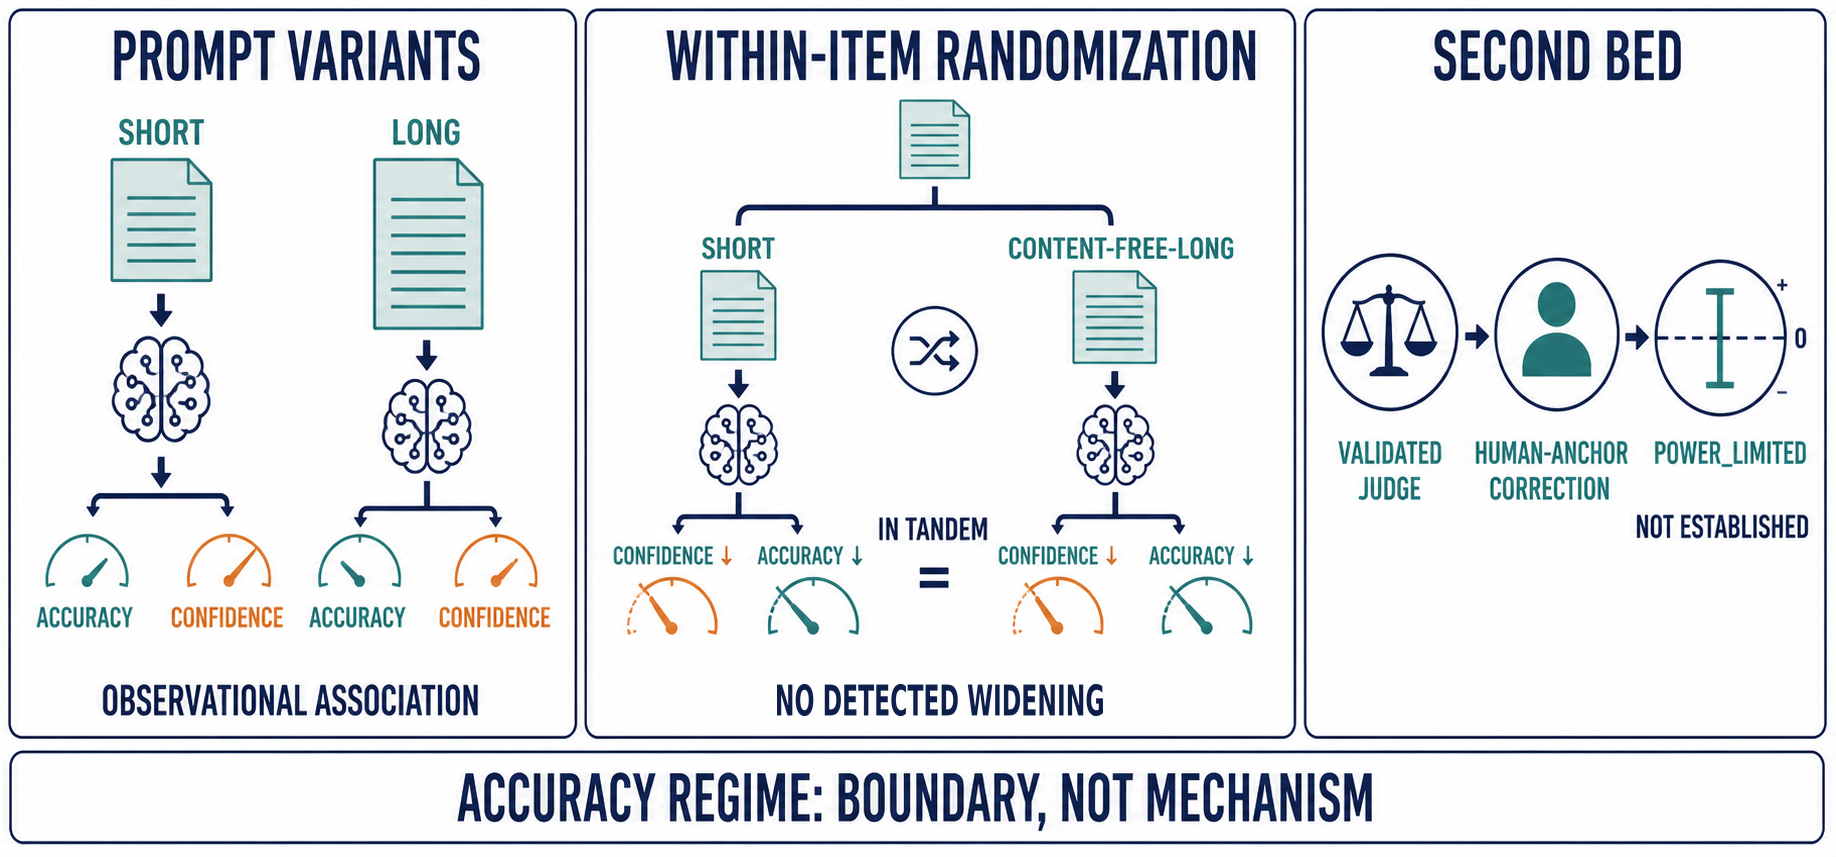
\includegraphics[width=\linewidth]{figures/calibration_teaser_refine6_r240_banner.png}
\caption{Measurement narrative.  As prompt length increases across prompt-length
variants, accuracy falls faster than confidence and the signed confidence--accuracy
gap is associated with length; a within-item randomized intervention shows length
lowers confidence and accuracy in tandem while the signed gap shows no detected
widening, bounded to $[-0.052,+0.039]$
(Table~\ref{tab:length-intervention}).  The middle panel's banner is shorthand for
that preregistered \textsc{not\_identified} verdict---no widening was detected at the
$+37$-token intervention dose---and not a claim that a causal widening has been ruled
out.  On the second bed,
the validated judge supplies an uncorrected read before human-anchor correction; the
corrected transportability conclusion is \textsc{power\_limited}.  The separate
difficulty strip summarizes the observed point-estimate boundary and makes no
mechanism claim.  This conceptual figure contains no generated experimental values.}
\label{fig:teaser}
\end{figure}

\begin{table}[t]
\centering
\caption{Within-item length-intervention result ($N{=}400$ paired problems, bed~1
GSM8K).  Arms share each base prompt: \textsc{Short} is the base,
\textsc{Long} adds 37 uniform tokens, and \textsc{Random} adds a $0..55$-token dose.
Within-item $\textsc{Long}-\textsc{Short}$ and $\textsc{Random}-\textsc{Short}$
deltas use paired per-problem outcomes, fixed uniform schedule~A
($\mathrm{NFE}{=}64$), content-free redundant filler, and a predeclared 100-item
gate with $0/200$ drift (seed $20260824$).  Adding content-free length lowers confidence
and accuracy in tandem; the signed gap is $\Delta\mathrm{SCE}=-0.0075\ [-0.052,+0.039]$
(preregistered verdict \textsc{not\_identified} --- no detected widening, interval
excludes the $+0.2227$ observational magnitude but not a small positive effect).
The co-primary family: ECE and adaptive-ECE show no detected widening
($[-0.014,+0.055]$ and $[-0.032,+0.046]$), while Brier
($+0.0213\ [0.011,0.031]$) and NLL ($+0.0452\ [0.024,0.067]$) worsen significantly.}
\label{tab:length-intervention}
\footnotesize
\setlength{\tabcolsep}{3pt}
\begin{tabular}{lccccc}
\toprule
quantity & Short & Long & Random & $L{-}S$ & $R{-}S$\\
\midrule
$\Delta\mathrm{SCE}$ & $-0.0724$ & $-0.0799$ & $-0.0861$ & $-0.0075\ [-0.052,0.039]$ & $-0.0137\ [-0.065,0.035]$\\
confidence & $0.630$ & $0.543$ & $0.574$ & $-0.0875\ [-0.098,-0.076]$ & $-0.0562\ [-0.067,-0.046]$\\
accuracy & $0.703$ & $0.623$ & $0.660$ & $-0.0800\ [-0.125,-0.033]$ & $-0.0425\ [-0.088,0.003]$\\
ECE & $0.0889$ & $0.1154$ & $0.1276$ & $+0.0264\ [-0.014,0.055]$ & \\
adaptive-ECE & $0.1153$ & $0.1248$ & $0.1226$ & $+0.0095\ [-0.032,0.046]$ & \\
Brier & $0.1922$ & $0.2135$ & $0.2245$ & $+0.0213\ [0.011,0.031]$ & \\
NLL & $0.5723$ & $0.6175$ & $0.6499$ & $+0.0452\ [0.024,0.067]$ & \\
\midrule
dose slope/tok & \multicolumn{5}{c}{$+0.0009\ [-0.002,+0.004]$ (cluster; see note)}\\
dose-bin $\Delta\mathrm{SCE}$ & \multicolumn{5}{c}{$\{-0.073,-0.126,-0.081,-0.057\}$ at dose $\{0,12,30,48\}$}\\
\bottomrule
\end{tabular}
\normalsize%
\setlength{\tabcolsep}{6pt}
\begin{minipage}{\linewidth}\small\emph{Within-item $L{-}S$ and $R{-}S$ deltas are per-problem cluster-bootstrap contrasts
($R{=}2000$ per problem seed $20260824$; points: $+0.0264$, $+0.0095$, $+0.0213$, $+0.0452$).
The $\textsc{Random}$ arm is the predeclared $0..55$-token uniform-dose arm, drawn
once per problem at the r198 predeclared seed.  The dose-response slope is a
per-problem paired regression (not a naive per-decode i.i.d.\ fit): the response is
$\Delta\mathrm{SCE}$, the predictor is the realized RANDOM-arm dose, and the
problem-cluster bootstrap clusters all three arms of the same problem on the same
resample, so the repeated-arm dependency is carried inside the cluster instead of
inflating the effective sample size of the SE computation.  A naive per-decode
(i.i.d.) fit of the signed-gap dose-response gives $+0.0022$/token ($p{=}0.0098$); this
naive per-decode model suffers from repeated-arm dependency (L arm draws the same
problem-content seed effects across its per-item doses) and uses the wrong
inference base, which renders the naive positive slope a multiplicity/i.i.d.-SE
artifact.  Heterogeneity beyond a linear-dose trend is already accounted for by the problem-cluster pairing: each problem carries
its own base level implicitly, which the fitted intercept
($-0.109$ with bootstrap interval $[-0.196,-0.025]$)
absorbs rather than indicating a content-free violation.  The paired-cluster estimate eliminates the heterogeneity
source: the per-problem cluster-bootstrap slope is $+0.0009$/token (95\% bootstrap
interval $[-0.002,+0.004]$, two-sided bootstrap $p{=}0.535$).  At the realized mean dose of $25.2$ tokens the fitted model
predicts a $\Delta\mathrm{SCE}$ shift of $+0.023$, inside the $R{-}S$ contrast CI
$[-0.059,+0.033]$ (per-decode cluster resampling; the per-item run tabulated in the
$R{-}S$ column above gives $[-0.065,+0.035]$, and $+0.023$ lies inside both);
the dose-bin means also do not trend monotonically.  Thus the
clustered dose slope is consistent with the preregistered \textsc{not\_identified}
verdict; we therefore read the naive positive slope as a multiplicity/i.i.d.-SE
artifact, not as a dose effect.  All intervals in this table are bootstrap
percentile intervals ($R{=}2000$, per-problem cluster resampling) under the
predeclared co-decision on the $L{-}S$ family.  ``---'' marks a metric kept
descriptive because the within-item contrast
was not part of the predeclared co-decision for that arm.}
\end{minipage}
\end{table}

\section{Two-component read on a second bed (MATH500)}
\label{sec:calib:bed2}

On a second, harder bed (MATH500, $n=400$, same decoder), the correctness label
requires a validated matcher for free-form prose finals (the \emph{judge v2},
\S\ref{sec:judge}).  Under the post-repair, label-aligned v2 judge
(Table~\ref{tab:judge-validation}), the primary v2 composite read is a
two-component estimate with a conservative $k{=}0$ (se-bias floor) interval,
positive and excluding zero:
\[
\Delta\mathrm{SCE}_{2,\mathrm{v2}}=+0.2382
\quad [0.1639,0.3125].
\]
This value is the designated second-bed v2 estimate; Table~\ref{tab:convention}
also reports an \emph{isin}-cluster bootstrap lens on the same datum
($+0.2308\ [0.1588,0.307]$) as a separately-named sensitivity, never as a competing
``same v2 point.''  Table~\ref{tab:convention} collects
every judge convention and its read (primary v2 row~3, lenient row~2); the
human-anchor-corrected read is shown here explicitly because it carries the
reporting-layer conclusion
\[
\Delta\mathrm{SCE}_{2,\mathrm{corr}}=+0.1606\quad [-0.059,+0.380],
\]
which contains zero.  \textbf{Sensitivity designation:} because the 30 human anchors
are purposive (not a probability sample), this interval is an anchor-dependent
design sensitivity interval, not a classical repeat-sampling confidence interval; a
fully-upgraded CI requires the predeclared FULL-193 two-strata probabilistic human
annotation (future work).  Figure~\ref{fig:gap} plots the decomposition (panel~a) and the
cross-bed reads with their intervals (panel~b).  The honest reporting-layer read is
\emph{POWER\_LIMITED} (limited by human anchor volume, not GPU).  The
v2 estimate is an uncorrected read, not a proven bound: the sign of full-bed
judge error is not identifiable from the purposive anchor.  Neither ``transportable
positive'' nor ``collapse'' is citable until an expanded, two-layer human anchor
pins the corrected estimate; Table~\ref{tab:judge-validation} separates the
fragility-lineage diagnostics from the post-repair v2-final audit.

The current cross-bed grade is \emph{POWER\_LIMITED}: the uncorrected judge reads and
the human-anchor correction lead to different inferential conclusions, and
$n_{\text{beds}}=2$ cannot establish general transportability.  We therefore do
\emph{not} report the composite as a settled transportable read
(in the causal-transportability sense of \citealp{pearl2014transportability}
this two-bed design does not satisfy the needed sampling/selection conditions); we
report each judge convention by name while awaiting an expanded human-label set.

The \emph{confidence} component is label-free and thus immune to the judge issue.
It is negative in both beds, but the cross-bed magnitudes shown in
Figure~\ref{fig:gap}a differ materially, so we report \emph{sign \mbox{consistency}
only}, not magnitude transportability.  It is
an exploratory, label-free byproduct and not a mechanism claim.

\begin{figure}[t]
\centering
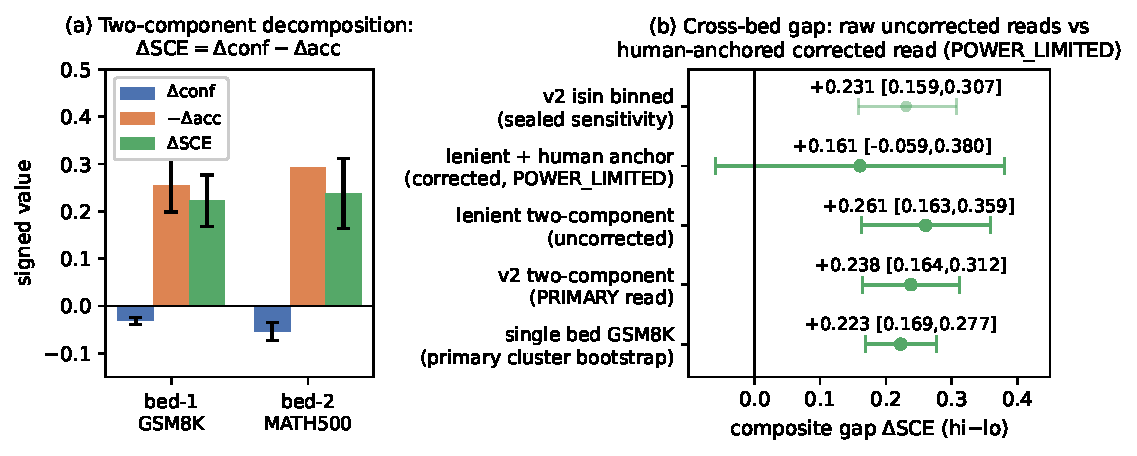
\includegraphics[width=\linewidth]{figures/calib_crossbed_gap.pdf}
\caption{Two-component decomposition (a) and cross-bed composite gap (b).  Panel (a):
$\Delta\mathrm{SCE}=\Delta\mathrm{conf}-\Delta\mathrm{acc}$ for the single bed and for
the second-bed v2 lens; on the single bed the accuracy- and confidence-side
shares are $114.1\%$ and $-14.1\%$, respectively, and sum to $100\%$ across opposing
signs.  Panel (b) designates the multiplicity-preserving
per-problem cluster interval as the primary single-bed read; the sealed isin interval
is retained only as a sensitivity artifact.  The primary v2 two-component read
($+0.2382$), its \emph{isin}-cluster sensitivity lens ($+0.2308$), and the lenient
two-component uncorrected reads exclude zero,
whereas the lenient human-anchor-corrected interval contains zero
(\textsc{POWER\_LIMITED}).}
\label{fig:gap}
\end{figure}

\section{Outcome-stratified sensitivity within GSM8K (corrected bootstrap)}
\label{sec:calib:control}

To check whether the within-bed composite is difficulty-sensitive, we sliced the
frozen single bed (GSM8K $g3\_main$ A/B', $n{=}1{,}948$, 974 problems) by per-problem
accuracy (the table's ``acc'' stratification variable) and recomputed the same estimator with a \emph{multiplicity-preserving}
per-problem cluster bootstrap \citep{davison1997bootstrap} (Table~\ref{tab:tiers}):

\begin{table}[t]
\centering
\caption{Outcome-stratified sensitivity within GSM8K (multiplicity-preserving
per-problem cluster bootstrap; primary CI convention throughout).  The rows are
nested per-problem accuracy regimes ($\mathrm{all}\supset\mathrm{low\text{-}acc}\supset\mathrm{acc{=}0}$),
not a partition and not an exogenous difficulty control.  Takeaway: point estimates
decrease across these outcome-defined subsets; at the accuracy floor,
$\Delta acc\equiv0$ by construction, so the composite equals
$\Delta\mathrm{conf}$ mechanically rather than empirically.  This is an
acc-regime-driven limitation and boundary, not a demonstrated difficulty trend or a
reproduction of the second-bed null.  Confidence is sign-consistent only; the sealed
isin bootstrap is a sensitivity analysis, not a parallel main read.}
\label{tab:tiers}
\begin{tabular}{lccc@{\hspace{1.2em}}c}
\toprule
tier & $n_{\mathrm{prob}}$ & acc & $\Delta\mathrm{conf}$ & composite gap [95\%]\\
\midrule
all        & 974 & 0.69 & $-0.0314$ & $+0.2227\;[+0.169,+0.277]$\\
low-acc ($acc\le q_{33}$) & 415 & 0.28 & $-0.0131$ & $+0.0551\;[-0.002,+0.107]$\\
acc $=0$ & 184 & 0.00 & $-0.0202$ & $-0.0202\;[-0.040,+0.001]$\\
\bottomrule
\end{tabular}
\end{table}

\section{Experimental setup}
\label{sec:setup}

\paragraph{Beds.}
Table~\ref{tab:bed-design} separates the two evaluation beds, sampling units,
prompt-length strata, and decode plans.  Bed~1 pairs GSM8K
\citep{cobbe2021gsm8k} with LLaDA-8B-Instruct \citep{nie2025large}; bed~2 uses the
same decoder on the first 400 MATH500 problems \citep{hendrycks2021math}, with
\texttt{decode\_id} equal to the problem index in
\nolinkurl{data/math500/test.jsonl}.

\begin{table}[h]
\centering
\caption{Evaluation-bed design ledger.  Takeaway: bed~1 is a paired crossover over
prompt-length extremes, whereas bed~2 has one decode per problem; counts, thresholds,
and decode schedules are reported separately rather than pooled across beds.}
\label{tab:bed-design}
\small
\begin{tabularx}{\linewidth}{@{}>{\raggedright\arraybackslash}p{0.10\linewidth}>{\raggedright\arraybackslash}p{0.39\linewidth}X@{}}
\toprule
bed & corpus, model, and sampling unit & prompt-length strata and decode plan \\
\midrule
1 & GSM8K + LLaDA-8B-Instruct; \texttt{g3\_main} A/B$'$ paired crossover; 1,948 decodes from 974 problems ($t1$ excluded: 608 / 304) & $t0{\le}62$: 672 / 336, mean 53.1, med.\ 54 tok; $t2{\ge}80$: 668 / 334, mean 98.6, med.\ 92 tok \\
2 & first 400 MATH500 problems; same decoder; one decode per problem & $t0{\le}48$: 134; $t1$: 130; $t2{\ge}77$: 136; A arm uses $\mathrm{NFE}{=}64$, schedule $(8,8,8,8,8,8,8,8)$ \\
\bottomrule
\end{tabularx}
\normalsize
\vspace{2pt}
\begin{minipage}{\linewidth}\small\emph{Decode-plan expansion (bed~1 observational crossover).}  Each of
the 974 problems in the frozen GSM8K \texttt{g3\_main} A/B$'$ pool is decoded twice
(once each under the crossover's A and B$'$ variants, $1{,}948 = 2\times974$ decodes);
the pairing is within-problem, allocating no randomization between arms.  The
observational tertile contrast is a post-hoc partition by realized prompt length:
$t0{:}672$ decodes are the 336 problems with prompt length $\le 62$ tokens
(mean 53.1, med.\ 54; 672$=2\times336$ decodes); $t1{:}608$ decodes are the 304
problems with prompt length in $(62, 80)$ tokens ($608=2\times304$; excluded from
the t0/t2 contrast by the predeclared design); $t2{:}668$ decodes are the 334
problems with prompt length $\ge 80$ tokens (mean 98.6, med.\ 92;
$668=2\times334$).  Selection by realized length is acknowledged post-hoc: the A/B$'$
crossover does not manipulate length, so content, format, and difficulty may co-vary
with the strata; the within-item randomized intervention
(Table~\ref{tab:length-intervention}) is the load-bearing causal design.
Bed~2 (MATH500) uses one decode per problem; ``first 400'' is the frozen
predeclared sample frame, not a post-hoc selection.
\end{minipage}
\end{table}

\paragraph{Estimator and interval.}
For each length set, confidence is mean commit-step confidence and correctness is
mean accuracy; therefore $\Delta\mathrm{SCE}=\Delta\mathrm{conf}-\Delta\mathrm{acc}$
is an identity, not a new estimator.  Primary intervals use a per-problem cluster
(multiplicity) bootstrap with $R=2000$, percentile 2.5/97.5 endpoints, and seed
20260824, implemented in \nolinkurl{scripts/r167/bootstrap_core.py}.

\paragraph{Judge and reporting layer.}
Judge v2 gives priority to explicit final-answer delimiters---balanced
$\backslash$boxed, display math, inline math, then \texttt{\#\#\#\#}-style markers---
before treating raw prose as a candidate.  It is validated against 30 human anchors
and a constructed oracle (Table~\ref{tab:judge-validation}).  Every cross-bed report
then receives the three-state \textsc{support}/\textsc{power\_limited}/%
\textsc{not\_measured} grade under the V-gate.

\section{The validated judge (v2)}
\label{sec:judge}

The MATH500 finals are free-form prose with a final $\backslash$boxed answer.  A judge
that feeds the whole prose tail to a LaTeX parser silently builds a bogus product of
undetermined symbols.  The frozen pre-repair lenient-judge snapshot is a
fragility-lineage diagnostic, not a v2-final measurement.  The v2 judge prioritizes
explicit final-answer delimiters (balanced
$\backslash$boxed, then display, then inline groups, then \texttt{\#\#\#\#}-style \mbox{markers})
before ever treating the raw prose as a candidate.  Table~\ref{tab:judge-validation}
separates the pre-repair diagnostic, constructed-oracle validation, and post-repair
human audit.  Both apparent false accepts in the pre-repair workbook are
machine-verified human mislabels whose boxed answer equals gold exactly.  That the
sampling anchor set contains such human mislabels matters for the pair-bias
correction $\hat b$ (Table~\ref{tab:convention}, row~1): the two mislabels were
corrected after machine verification, and the residual anchor-level mislabel rate
after repair is $0/30$ on the spot, so the correction's input labels are taken as
clean; any uncorrected residual anchor error would enter $\hat b$ directly and is
audited here, not assumed away.  To make the Table~\ref{tab:judge-validation} counts
reconstructible, each count is named by its judge \emph{and} its human column, since
the two figures on the pre-repair row come from two different judges on the same
$30$ items.  (i)~The pre-repair spot ledger
\nolinkurl{results/r83_branchA_launch/spot_labelled.json} is the authoritative source
for the failure mode: against the pre-repair human column the pre-repair judge
rejects the $7$ items whose label reads ``correct'' ($\mathrm{FR}{=}7$), accepts only
decodes $366$ and $70$ (both of which that column also calls correct, so
$\mathrm{FA}{=}0$), and therefore agrees on $23/30$ items.  (ii)~The
$0.933=28/30$ figure is the \emph{v2} judge scored against that same pre-repair
column in \nolinkurl{results/r109_judge_v2_validate.json}: $\mathrm{FR}{=}0$ with $2$
apparent false accepts, namely decodes $319$ and $59$.  Those two are the
machine-verified anchor mislabels---the extracted finals equal the
\nolinkurl{data/math500/test.jsonl} golds ($-128$ and $5$) exactly, so the human
labels, not the judge, were wrong, and they were repaired to ``correct'' in
\nolinkurl{processing/anchors/anchor_labels.csv}.  Against the repaired column the v2
audit is $30/30$ with $0$ false rejects and $0$ false accepts
(Table~\ref{tab:judge-validation}, row ``post-repair v2'').  The $7/30$ FR and the
$0.933$ agreement are thus not two views of one reconciliation, and neither number
is a v2-final measurement of the pre-repair judge.

\begin{quote}\small\raggedright
\textbf{2$\times$2 confusion tables.} Rows = judge verdict, columns = human
reference; each cell is the count over the same $30$-item anchor spot.
\textit{Pre-repair judge vs.\ pre-repair labels}
$\begin{smallmatrix}2&0\\7&21\end{smallmatrix}$ ($TP{=}2,\ FA{=}0,\ FR{=}7,\
TN{=}21$; agreement $23/30$).
\textit{v2 judge vs.\ pre-repair labels}
$\begin{smallmatrix}9&2\\0&19\end{smallmatrix}$ ($TP{=}9,\ FA{=}2$ on the anchor
mislabels $\{59,319\}$, $FR{=}0$, $TN{=}19$; agreement $28/30$).
\textit{v2 judge vs.\ repaired labels}
$\begin{smallmatrix}11&0\\0&19\end{smallmatrix}$ ($TP{=}11,\ FA{=}0,\ FR{=}0,\
TN{=}19$; agreement $30/30$).
The apparent $7/30$ vs.\ $28/30$ gap is therefore two different judges on the same
pre-repair human column, made explicit by cell count; it is not an internal
inconsistency of this paper.
\end{quote}

\begin{table}[h!]
\centering
\caption{Judge-validation ledger.  Takeaway: the pre-repair lenient snapshot exposes
the prose-tail failure mode, whereas the post-repair v2 judge passes both the
constructed-oracle check and the complete hand-labelled spot audit; pre-repair
diagnostics are not v2-final measurements.}
\label{tab:judge-validation}
\begin{tabularx}{\linewidth}{@{}>{\raggedright\arraybackslash}p{0.20\linewidth}>{\raggedright\arraybackslash}p{0.22\linewidth}X@{}}
\toprule
stage & audit set & recorded result \\
\midrule
pre-repair lenient & 30-item hand spot & fragility-lineage snapshot: $7/30$ false rejects (FR) and $23/30$ agreement for the pre-repair judge; the v2 judge on the \emph{same} 30 pre-repair labels agrees $0.933=28/30$, its two disagreements being the anchor mislabels (a different judge's agreement figure, not the same count; \S\ref{sec:judge}) \\
constructed oracle & 500 golds $\times$ self + perturbed & maximum per-tier $\epsilon\le0.05$; oracle independence held \\
post-repair v2 & 30-item hand spot & 0 false rejects; 30/30 agreement \\
% r240 layout audit: without this the single-line "post-repair v2" row abuts the
% four-line stage cell below it and the two rows read as one entry.
\addlinespace
pre-repair accepted audit (v2 vs pre-repair labels) & 2 apparent false accepts (decodes 319, 59) & both are machine-verified human mislabels \\
\bottomrule
\end{tabularx}
\end{table}

\section{Related work}
\label{sec:related}

\paragraph{Decoder family.}
Masked text diffusion includes structured, simplified, ratio-estimation, and
reparameterized discrete formulations
\citep{austin2021structured,shi2024simplified,lou2024discrete,zheng2023reparameterized}
and the LLaDA family \citep{nie2025large,nie2026improved}.  Variable-length or
confidence-guided decoders \citep{li2025beyond,sun2026dystruct,wang2026reversible}
and continuous language-flow alternatives \citep{hu2026elf} delimit our fixed
single-bed setting: we make no decoder-generality claim.

\paragraph{Calibration.}
Language-model confidence is a calibration-relevant observable
\citep{kadavath2022language}.  We study the signed confidence--accuracy gap
$\mathrm{SCE}=\mathbb{E}[\mathrm{conf}]-\mathbb{E}[\mathrm{acc}]$ (a signed
calibration-in-the-large quantity, distinct from the binned expected calibration
error) and its length contrast with per-problem cluster-bootstrap inference
\citep{davison1997bootstrap}.  For completeness Table~\ref{tab:length-intervention}
also reports expected calibration error (ECE) with fixed 10 equal-width bins
\citep{guo2017calibration}, adaptive (equal-mass) ECE
\citep{naeini2015obtaining}, Brier score \citep{brier1950verification}, and negative
log-likelihood; each is computed on the same per-problem confidence and correctness
events as $\mathrm{SCE}$.  Because $\mathrm{SCE}$ is a first-order mean gap, it is
not a substitute for a full calibration curve, and we make no equivalence claim to
ECE or temperature scaling; we report them as companion descriptors with the
definitions above.

\paragraph{Answer matching.}
Free-form mathematics finals require an answer-matching judge.  Our judge-and-human
audit is anchored in GSM8K verifier and matching methodology
\citep{cobbe2021gsm8k}; the audited per-stratum failure ledger, including the
separation of pre- and post-repair snapshots, is our reusable contribution.

\paragraph{Positioning.}
To our knowledge, prior work has not reported this exact two-component length
contrast inside a masked-diffusion decoder with a problem-multiplicity-preserving
bootstrap, an audited judge, and a within-item causal check that separates the
length association from a length mechanism.  We report a boundary limited by the
second bed, not a transportable law; our single-bed length claim is scoped to the
within-item causal check on this bed and does not extend to nearest-neighbor
(non-masked-diffusion) decoders, which remain an open same-bed contrast.
Outcome-stratified controls additionally require
positivity/common-support and coefficient-interpretation caution
\citep{petersen2012positivity,westreich2013table2fallacy}.

\section{Limitations of this calibration read}
\begin{itemize}
\item Single-bed anchor.  The uncorrected cross-bed read and its current
human-anchor correction are reported in Table~\ref{tab:convention}; the corrected
read is \emph{POWER\_LIMITED}.  Four-state grading awaits the predeclared expanded
two-layer human-label set, and two beds are not universal.  Neither
``transportable-positive'' nor ``collapse'' is citable until then.
\item No single-bed control arm is included in the second bed, so we cannot fully separate
cross-task transportability from a second-bed main effect (difficulty reconciliation is
not clean; interpreting tier-stratified associations as the effect carries the usual
coefficient-over-interpretation \citep{westreich2013table2fallacy} and positivity/coverage
\citep{petersen2012positivity} cautions).
\item The within-bed outcome-stratified sensitivity shows a \emph{point-estimate}
decrease through zero across nested accuracy subsets (Table~\ref{tab:tiers},
\S\ref{sec:calib:control}); the CIs
retain significance only at the all subset under the primary cluster bootstrap.
At the accuracy floor ($acc{=}0$) $\Delta acc\equiv0$ by construction, so the equality
$\Delta\mathrm{SCE}=\Delta\mathrm{conf}$ there is mechanical; only the low-accuracy
tier can move $\Delta acc$, and under the wide primary intervals neither the collapse
nor its flatness is statistically pinned.  We therefore report the collapse as an
acc-regime-driven \emph{limitation} and boundary, not a mechanism claim --- and we do
not use control-arm CI non-significance to dismiss the difficulty explanation, as
interpretation in either direction is convention-sensitive.
\item \emph{Content-free length only.}  The within-item manipulation adds
\emph{semantically null} redundant filler (validity gate: $0/200$ drift), whereas
the observational contrast varies \emph{natural} prompt lengths that co-vary with
content and difficulty.  The intervention therefore identifies the effect of
content-free length on this bed, but does not exclude a length mechanism that acts
through content-bearing or difficulty-changing length; a content-bearing-length arm
is left as future work.
\item The confidence component is reported sign-consistently only; its cross-bed
magnitude difference is summarized with Figure~\ref{fig:gap}a and
Table~\ref{tab:tiers}.
\end{itemize}

\section{Conclusion}
On GSM8K, the supported result is an \emph{observational} association across
prompt-length variants, decomposed into opposing accuracy and confidence components
(Figure~\ref{fig:gap}a).  The within-item randomized experiment
(Table~\ref{tab:length-intervention}) finds that content-free length lowers confidence
and accuracy together but does not detect a widening of their signed gap
(\textsc{not\_identified}).  Its interval excludes the observational magnitude without
ruling out a small positive effect; the observational contrast therefore does not
establish a length$\to$gap mechanism.  Cross-bed transport remains
\textsc{power\_limited}.  The reusable outputs are the predeclared within-item check and
the judge-audit trail that separates pre-repair diagnostics from the validated v2
measurement.  The outcome-defined accuracy-regime analysis is a boundary condition, not
a reproduction of a second-bed null.  Remaining work includes the FULL-193 human fill,
an exogenous difficulty control, a second model, and a same-bed nearest-neighbor
(non-masked-diffusion) contrast.

% P5_MAIN_TEXT_END
\label{p5:main-text-end}

\begingroup
% Keep references readable while avoiding a bibliography-only orphan page.
% This remains larger than the common 8pt conference-reference setting.
\fontsize{8.5}{9.4}\selectfont
\setlength{\bibsep}{0pt}
\bibliographystyle{iclr2026_conference}
\bibliography{refs}
\endgroup

\appendix

\section{Adjudication protocol: minimum decisive label set (MDLS-101) and one-count rule}
\label{sec:mdls}

The decisive three-state read needs \emph{both} strata of the predeclared two-layer
anchor: Layer-1 = the judge-accepted set (defines \textsc{fa}$_t$ =
$P(\mathrm{human=incorrect}\mid\mathrm{judge\;accepted})$) and Layer-2 = the
judge-rejected sample (defines \textsc{fr}$_t$ =
$P(\mathrm{human=correct}\mid\mathrm{judge\;rejected})$).
Labeling Layer-2 alone leaves \textsc{fa} undefined and the read \emph{invalid}.
Table~\ref{tab:anchor-design} collects the complete anchor-count design, the interval
construction, and the decision gates.  The interval construction is named explicitly.
The $t0$--FR count is monotone-benign and cannot flip the
knife-edge rule.

\paragraph{Citable value is judge-convention-dependent (decode-398 single-point leverage).}
The folded citable value (Table~\ref{tab:convention}, row~1) is the lenient-judge
read with a human-anchor pair-bias correction, and it rides on the repaired decode 398
label (gold ``Navin''; prose final-answer credit).  The answer-aware \textbf{v2} judge
accepts that case and shows zero observed disagreement on the $t0\cup t2$ gradient
subset (Table~\ref{tab:convention}, panel~b), so the zero is a floor, not a precision
estimate.  Rows~3--5 propagate the declared sampling
ladder and show the flip to \textsc{power\_limited}; row~6 records the single-source
fragile-gold look-back.  Thus row~1 remains the citable value, while the v2 rows remain
convention sensitivities until accepted-stratum annotation publishes their FA/FR
lists.  The full-bed shift reported in the caption confirms that the judge update is a
two-term result.

\textbf{Honest blind-spot and a certified hidden FA.}  The accepted-set blind spot
is not hypothetical: decode 120 ($t1$; gold ``even'', model boxes ``neither'';
composition always even) is a zero-label-provable hidden false accept.  As summarized
in Table~\ref{tab:anchor-design}, this case invalidates the assumed-clean MDLS route,
while the full-fill tolerance envelope remains a separate sensitivity.  Hence a
decisive SUPPORT must be certified with the accepted-stratum FA ceiling.  Neither
route replaces the real human fill: no model-generated pseudo-label is admitted into
the decisive read.

% r240 layout audit: [!b] parked this float at the foot of the page that opens the
% "Data and reproducibility" list, so the lead-in "The source bundles are:" was left
% dangling above it and the list itself was pushed to the next page.  [t] keeps the
% table on the page after its \S A citation without splitting that sentence.
\begin{table}[t]
\centering
\caption{Anchor design and count-form decision ledger.  Takeaway: MDLS-101 is only a
SUPPORT route under an assumed-clean accepted stratum; the certified hidden false
accept violates that assumption, so a decisive read requires the accepted-stratum
ceiling or the full two-layer human fill.}
% The grade names are long unbreakable \textsc runs; justifying this note stretches
% its first line, so it is set ragged-right.
\begin{minipage}{\linewidth}\small\raggedright\emph{Grade-symbol clarification: this ledger uses
the plain three-state
\textsc{support}/\textsc{power\_limited}/\textsc{not\_measured} set defined in
\S\ref{sec:intro}; every instance of the obsolete ``SUPPORT*'' badge that earlier
drafts showed has been collapsed to \textsc{support} (defined identically:
the predeclared audit passed), and any route that previously claimed SUPPORT*
under an unmeasured accepted stratum is now explicitly labelled \textsc{power\_limited}
(row ``accepted-stratum blind spot'' below).  The plain
\textsc{support} grade is reserved for a measured two-layer fill (FULL-193)
and is not awarded to the current citable value.}\end{minipage}
\vspace{2pt}
\label{tab:anchor-design}
\begin{tabularx}{\linewidth}{@{}>{\raggedright\arraybackslash}p{0.24\linewidth}>{\raggedright\arraybackslash}p{0.27\linewidth}X@{}}
\toprule
quantity & declared value & role / interpretation \\
\midrule
Layer-1 reuse anchors & 11 of 103 accepted; $t0/t1/t2=7/3/1$ & pins \textsc{fa}$=0$ only on the reuse frame \\
Layer-2 rejected anchors & 90 total; 30 per tertile & estimates \textsc{fr} \\
MDLS-101 fill & $101=11+90$ labels & SUPPORT route under assumed-clean accepted-set \textsc{fa} \\
FULL-193 fill & $193=103+90$ labels & complete two-layer human fill \\
primary two-component interval & $+0.2382\ [0.1639,0.3125]$ & v2 point; Table~\ref{tab:convention}, row~3 \\
$t2$--FR knife edge & 30 items; $\le3$: SUPPORT; $\ge4$: POWER\_LIMITED & authoritative count-form V-gate \\
accepted-stratum blind spot & 92 outside reuse; certified \textsc{fa}$\ge1$ & one hidden false accept already breaks MDLS-101 SUPPORT \\
FULL-193 tolerance & $k\le5$: SUPPORT; $k\ge6$: NOT\_MEASURED & label-free hidden-\textsc{fa} envelope \\
current count-form FA gate & $n_{\mathrm{incorrect}}=19$; $\lfloor0.05\times19\rfloor=0$ & zero-count statement, not a calibration proof \\
\bottomrule
\end{tabularx}
\end{table}

\paragraph{Explicit count, not a black-box sixth participant.}
Every stratum that governs the correction and the V-gate is enumerated by an
explicit count in the supporting tables, so the audit is recoverable from counts
alone and the judge is never treated as an opaque aggregate participant.  Each label
set is declared with its own denominator: the 30-item hand spot
(Table~\ref{tab:judge-validation}), its $t0\cup t2$ gradient 20-subset and the
full-30 rule-of-three bounds \citep{vanbelle2008rules}
(Table~\ref{tab:convention}, panel~b), and the Layer-1
and Layer-2 anchor sets together with the MDLS-101 and FULL-193 fills
(Table~\ref{tab:anchor-design}).  The frozen labels that ground these counts are
stored at \nolinkurl{processing/anchors/anchor_labels.csv}; the correction and its
uncertainty follow from that file together with the per-stratum totals in those
tables, without any recourse to an aggregate ``sixth'' quantity.  The decisive read
thus remains \textsc{power\_limited} until the predeclared FULL-193 probability fill
expands the labels; no number in this paper is backed by an un-enumerated label.

% r240 layout audit: Table 5 takes the page top; keeping this one at the page foot
% packs the appendix without re-creating the dangling "The source bundles are:" line.
\begin{table}[!b]
\centering
\caption{Reporting-layer sensitivity of the second-bed MATH500 composite gap to judge
convention and anchor-count uncertainty.  Takeaway: the citable verdict is
\emph{judge-convention-dependent}.  Under the lenient judge with the $30$-anchor
pair-bias correction (row~1) the read is \textsc{power\_limited}
($+0.1606\ [-0.059,+0.380]$).  Under the validated v2 judge, the measured anchor
pair-bias is $0$ (v2 agrees with all $30$ human anchors; $0$ discordant), so the
v2 read (row~3) is positive and excludes $0$ ($+0.2382\ [0.1639,0.3125]$).  We report
both honestly rather than fixing a single convention; rows~3--5 keep the v2 point and
vary the anchor-\emph{uncertainty} index $k\in\{0,1,2\}$; the $\sqrt{k}/10$
propagation is a conservative convenience bound on the purposive anchor, \emph{not}
an identified sampling standard error, with
$\mathrm{se_{bias}}(k)=\sqrt{k}/10$ where $k$ is the count of discordant anchors over a
$10$-per-tier $t_0\cup t_2$ gradient subset (row~1 is implicitly $k{=}1$).  Panel (b)
makes the denominator-sensitive audit explicit.}
\label{tab:convention}
\textit{(a) Convention sensitivity}\par\smallskip
\begin{tabularx}{\linewidth}{@{}r>{\raggedright\arraybackslash}Xll@{}}
\toprule
\# & convention / correction & composite gap [sens.\ int.] & read\\
\midrule
1 & lenient $+$ 30-anchor pair-bias correction (\textbf{citable}; $k{=}1$, $\mathrm{se_{bias}}{=}0.1$) & $+0.1606\;[-0.059,+0.380]$ & \textsc{power\_limited}\\
2 & lenient, uncorrected & $+0.2606\;[0.1625,0.3587]$ & excl.\ $0$\\
3 & \textbf{v2 answer-aware, measured bias $0$ ($k{=}0$ se-bias floor); designated second-bed value} & $+0.2382\;[0.1639,0.3125]$ & excl.\ $0$\\
4 & v2 point, $k{=}1$ ($\mathrm{se_{bias}}=0.100$) sensitivity & $+0.2382\;[0.029,0.448]$ & sensitivity\\
5 & v2 point, $k{=}2$ ($\mathrm{se_{bias}}=0.141$) sensitivity & $+0.2382\;[-0.049,0.525]$ & \textsc{power\_limited}\\
6 & v2, fragile-gold verdicts corrected (single-source look-back) & $+0.2605\;[0.186,0.335]$ & sensitivity\\
7 & v2, \emph{isin}-cluster binned variant (0.2308; sealed fragility-lineage, NOT the two-component 0.2382; sensitivity only) & $+0.2308\;[0.1588,0.307]$ & excl.\ $0$\\
\bottomrule
\end{tabularx}
\smallskip
\textit{(b) Audit contrasts}\par\smallskip
\begin{tabularx}{\linewidth}{@{}>{\raggedright\arraybackslash}p{0.28\linewidth}>{\raggedright\arraybackslash}p{0.31\linewidth}X@{}}
\toprule
diagnostic & values & interpretation \\
\midrule
gradient-subset rule of three & $0/20$ observed; $3/20\approx0.15$ bound & $k{=}2$ ($\mathrm{se_{bias}}\approx0.141$) lies inside \\
full-anchor rule of three & $0/30$ observed; $3/30\approx0.10$ bound & $k{=}2$ lies outside; retained design denominator \\
judge gradient set & 20-item subset of the 30-anchor spot ($t_0/t_2{=}10{+}10$; $t_1$ excluded) & v2 zero observed disagreement on it \\
judge full-bed term & $0.3151\to0.2927$ & update is a two-term result \\
\bottomrule
\end{tabularx}
\end{table}

\section{Citable-value convergence and citation hygiene}
\label{sec:converge}

The reporting-layer citable value for the second-bed analysis is the
\emph{POWER\_LIMITED}, bias-corrected read (an anchor-dependent design sensitivity interval, not a repeat-sampling confidence interval):
\[
\Delta\mathrm{SCE}_{2,\mathrm{corr}}=+0.1606\quad [-0.059,+0.380]
\,.
\]

\paragraph{Explicit uncertainty propagation of the citable read.}
This estimate is an additive estimator of three random quantities,
$\Delta\mathrm{SCE}_{2,\mathrm{corr}}=\Delta\mathrm{conf}_2+(\mathrm{neg}\,\Delta\mathrm{acc}_2-\hat b)$.
Under independence its variance decomposes as
$\mathrm{se}^2=\mathrm{se}^2_{\mathrm{comp}}+\mathrm{se}^2_{\hat b}$.  The bed2
component standard error is $0.05005$ and the anchor-correction standard error is
$\mathrm{se}_{\hat b}{=}0.1$, which together reproduce the reported interval.  Here
$\mathrm{se}_{\hat b}(k)=\sqrt{k}/10$, where $k{=}1$ is the count of discordant
anchors over a $10$-per-tier $t_0\cup t_2$ gradient subset under the lenient judge
(the single divergent decode~398); the correction that suppressed two confirmed
human mislabels contributed approximately $80\%$ of the variance, so the
\emph{POWER\_LIMITED} verdict is driven by anchor uncertainty rather than by an
uninformative bed2 gap.  The verdict is judge-convention-dependent: under the
validated v2 judge the measured anchor pair-bias is $0$ (zero discordant anchors),
so the v2 read is positive and excludes $0$ ($+0.2382\ [0.1639,0.3125]$,
row~3 of Table~\ref{tab:convention}); the lenient-plus-correction read is the
conservative one we report (row~1).  A nested bootstrap is not run because the current
anchors are purposive; the probability-sample FULL-193 fill is the experiment that
would make the correction identifiable.

The uncorrected second-bed values in Figure~\ref{fig:gap}b and
Table~\ref{tab:convention} remain named convention sensitivities; neither is
presented as a proven bound or as the corrected point estimate.  The single-bed
estimate and interval in Figure~\ref{fig:gap}b remain the load-bearing zero-drift
anchor.

\paragraph{Count-form limitation on the minimal anchor.}
The current count-form V-gate is summarized in
Table~\ref{tab:anchor-design}: its FA threshold is \emph{unevaluable} as a
calibration proof because passing requires a zero count.  This does not change the
t2-FR knife-edge rule (it is
\emph{FR}-count, not \emph{FA}-count, and governs SUPPORT vs.\ POWER\_LIMITED); it
only sharpens the honesty of the minimal FA-based gate: FA quality there is
assumed-clean, not measured.  A measured FA gate requires the full fill or a larger
accepted-set sample.

\section*{Data and reproducibility}
Every headline number is linked to a frozen artifact and to the one-command reproducer
\texttt{python3} \nolinkurl{scripts/r167/reproduce_all_tables.py}.  Its report in
\nolinkurl{results/r167_reproduction_gate/} records 94 checks ($93$ direct passes plus
numbered ledger seams) and zero failures; the
machine-readable estimand map is \nolinkurl{processing/estimand_ledger_r881.csv},
materialized from \nolinkurl{scripts/r167/aggregate_meta.json}.  The source bundles are:
\begin{itemize}
\raggedright  % file paths are unbreakable \texttt runs; justifying them stretches the line
\item \nolinkurl{results/r37_data/} and \nolinkurl{results/r171_dacc_ci.json} ---
single-bed point estimates, primary multiplicity-bootstrap intervals, and the
component intervals and signed shares summarized in Figure~\ref{fig:gap}a;
\item \nolinkurl{results/crossbed_math500/} --- second-bed confidence, accuracy, and
composite inputs, including the primary v2 two-component read and the \emph{isin}-cluster sensitivity lens;
\item \nolinkurl{processing/anchors/anchor_labels.csv} --- frozen human-anchor labels and
post-repair v2 agreement;
\item \nolinkurl{results/r127_v2_harden/r127_v2_harden.json} --- the row-6
single-source fragile-gold look-back provenance;
\item \nolinkurl{results/r103_difficulty_matched_control.json} --- difficulty-tier
points, sample counts, and primary cluster intervals in Table~\ref{tab:tiers};
\item \nolinkurl{results/r200_length_intervention/decisive_result_r204.json} and
\nolinkurl{results/len_intervention/} --- within-item length-intervention
co-primary result and parquet data for Table~\ref{tab:length-intervention}
(predeclared in \nolinkurl{prereg/r198_length_intervention_prereg.md}).
\end{itemize}
The primary interval protocol is $R=2000$ resamples, percentile 2.5/97.5 CI,
seed 20260824, per-problem cluster (multiplicity) bootstrap via
\nolinkurl{scripts/r167/bootstrap_core.py}.  The sealed isin bootstrap is retained only
as a documented sensitivity (e.g.\ the row~7 v2 \emph{isin}-cluster lens on the second
bed); it is never mixed into the primary single-bed reading or presented as a second
primary v2 estimate.

\end{document}
